%\documentclass[a4paper,superscriptaddress,11pt]{quantumarticle}
\documentclass[aps,twocolumn,longbibliography,english,superscriptaddress,prr]{revtex4-1}
%\documentclass[a4paper,superscriptaddress,11pt]{article}
\pdfoutput=1
\usepackage[colorlinks=true,urlcolor=blue,citecolor=blue,linkcolor=blue]{hyperref}
\usepackage[T1]{fontenc}
%\usepackage[latin9]{inputenc}
\usepackage{amssymb}
\usepackage{tabularx}
\usepackage{upquote}
%\usepackage{multicol}
%\usepackage{caption}
\usepackage[plain]{algorithm}
\usepackage{algpseudocode}
\usepackage{rotating}
%\usepackage{cite}
\usepackage{booktabs}
%\usepackage{unicode-math}
%\usepackage{algorithm}% http://ctan.org/pkg/algorithm
%\usepackage{algpseudocode}% http://ctan.org/pkg/algpseudocode
\usepackage{xcolor}% http://ctan.org/pkg/xcolor
\makeatletter
\newsavebox{\@brx}
\newcommand{\llangle}[1][]{\savebox{\@brx}{\(\m@th{#1\langle}\)}%
  \mathopen{\copy\@brx\kern-0.5\wd\@brx\usebox{\@brx}}}
\newcommand{\rrangle}[1][]{\savebox{\@brx}{\(\m@th{#1\rangle}\)}%
  \mathclose{\copy\@brx\kern-0.5\wd\@brx\usebox{\@brx}}}
\makeatother

\usepackage{bbm}
\usepackage{jlcode}
\usepackage{graphicx, subfigure}
\usepackage{amsmath,color}
\usepackage{mathrsfs}
\usepackage{float}
\usepackage[normalem]{ulem}
\usepackage{indentfirst}
\usepackage{txfonts}
\usepackage{listings}
\usepackage[epsilon, tsrm, altpo]{backnaur}

\lstset{
    basicstyle=\ttfamily\footnotesize,
    numberstyle=\scriptsize,
    % numbers=left,
    backgroundcolor=\color{gray!10},
    frame=single,
    tabsize=2,
    rulecolor=\color{black!30},
    title=\lstname,
    escapeinside={(*}{*)},
    breaklines=true,
    breakatwhitespace=true,
    framextopmargin=2pt,
    framexbottommargin=2pt,
    extendedchars=true,
    inputencoding=utf8,
    columns=fullflexible,
}


\tolerance=1
\emergencystretch=\maxdimen
\hyphenpenalty=1000
\hbadness=1000

\makeatletter

%%%%%%%%%%%%%%%%%%%%%%%%%%%%%% User specified LaTeX commands.

%Journal reference.  Comma sets off: name, vol, page, year
\def\journal #1, #2, #3, 1#4#5#6{{\sl #1~}{\bf #2}, #3 (1#4#5#6) }
\def\pr{\journal Phys. Rev., }
\def\prb{\journal Phys. Rev. B, }
\def\prl{\journal Phys. Rev. Lett., }
\def\pl{\journal Phys. Lett., }
%\def\np{\journal Nucl. Phys., }


%%%%%%%%%%%%%%%%%%%%%%%%%%%%%%%%%%%%%%%%%%%%%%%%%%%%%%%%%%%%%%%%%%%%%%%%%%%%%%%%%%%%%%%%%%%%%%%%%%%%%%%%%%%%%%%%%%%%%%%%%%%%%%%%%%%%%%%%%%%%%%%%%%%%%%%%%%%%%%%%%%%%%%%%%%%%%%%%%%%%%%%%%%%%%%%%%%%%%%%%%%%%%%%%%%%%%%%%%%%%%%%%%%%%%%%%%%%%%%%%%%%%%%%%%%%%


%\usepackage{CJK}
%\usepackage[colorlinks, citecolor=blue]{hyperref}
\DeclareMathOperator*{\argmax}{arg\,max}

%%%%%% Shortcut related
\newcommand{\<}{\langle}
\renewcommand{\>}{\rangle}
\newcommand{\out}{{O}}
\newcommand{\inp}{{I}}
\newcommand{\pluseq}{\mathrel{+}=}
\newcommand{\minuseq}{\mathrel{-}=}
\newcommand{\vx}{{x}}
\newcommand{\vy}{{y}}
%%%%%% Convention related
\newcommand{\SWAP}{{\rm SWAP}}
\newcommand{\CNOT}{{\rm CNOT}}
\newcommand{\X}{{\rm X}}
\renewcommand{\H}{{\rm H}}
\newcommand{\Rx}{{\rm Rx}}
\renewcommand{\v}[1]{{\bf #1}}
\newcommand{\dataset}{{\mathcal{D}}}
\newcommand{\wfunc}{{\psi}}
\newcommand{\SU}{{\rm SU}}
\newcommand{\UU}{{\rm U}}
\newcommand{\thetav}{{\boldsymbol{\theta}}}
\newcommand{\gammav}{{\boldsymbol{\gamma}}}
\newcommand{\thetai}{{\theta^\alpha_l}}
\newcommand{\Expect}{{\mathbb{E}}}
\newcommand{\Tr}{{\rm Tr}}
\newcommand{\etc}{{\it etc~}}
\newcommand{\etal}{{\it etal~}}
\newcommand{\xset}{\mathbf{X}}
\newcommand{\fl}{\texttt{fl}}
\newcommand{\pdata}{\mathbf{\pi}}
\newcommand{\q}{\mathbf{q}}
\newcommand{\epdata}{\mathbf{\hat{\pi}}}
\newcommand{\gammaset}{\boldsymbol{\Gamma}}
\newcommand{\ei}{{\mathbf{e}_l^\alpha}}
\newcommand{\vtheta}{{\boldsymbol{\theta}}}
\newcommand{\sigmag}{{\nu}}
\newcommand{\sigmai}[2]{{\sigma^{#2}_{#1}}}
\newcommand{\qi}[1]{{q^{\alpha_{#1}}_{#1}}}
\newcommand{\BAS}{Bars-and-Stripes}
\newcommand{\circled}[1]{\raisebox{.5pt}{\textcircled{\raisebox{-.9pt} {#1}}}}

\newcommand{\qexpect}[1]{{\left\langle #1\right\rangle}}
\newcommand{\expect}[2]{{\mathop{\mathbb{E}}\limits_{\substack{#2}}\left[#1\right]}}
\newcommand{\var}[2]{{\mathop{\mathrm{Var}}\limits_{\substack{#2}}\left(#1\right)}}
\newcommand{\pshift}[1]{{p_{\thetav+#1}}}
\newcommand{\upcite}[1]{\textsuperscript{\cite{#1}}}
\newcommand{\Eq}[1]{Eq.~(\ref{#1})}
\newcommand{\Fig}[1]{Fig.~\ref{#1}}
\newcommand{\Tbl}[1]{Table~\ref{#1}}
\newcommand{\Sec}[1]{Sec.~\ref{#1}}
\newcommand{\App}[1]{Appendix \ref{#1}}
\newcommand{\bra}[1]{\mbox{$\left\langle #1 \right|$}}
\newcommand{\ket}[1]{\mbox{$\left| #1 \right\rangle$}}
\newcommand{\braket}[2]{\mbox{$\left\langle #1 | #2 \right\rangle$}}
\newcommand{\tr}[1]{\mathrm{tr}\mbox{$\left[ #1\right]$}}

\newcommand{\ra}[1]{\renewcommand{\arraystretch}{#1}}

%%%%%% Comment related
\newcommand{\red}[1]{[{\bf  \color{red}{LW: #1}}]}
\newcommand{\xred}[1]{[{\bf  \color{red}{\sout{LW: #1}}}]}
\newcommand{\blue}[1]{[{\bf  \color{blue}{JG: #1}}]}
\newcommand{\xblue}[1]{[{\bf  \color{blue}{\sout{JG: #1}}}]}
\newcommand{\material}[1]{\iffalse[{\bf  \color{cyan}{Material: #1}}]\fi}


\makeatother

\usepackage[english]{babel}

\begin{document}
\title{Instruction level automatic differentiation on a reversible Turing machine}

%\author{Jin-Guo Liu\thanks{cacate0129@iphy.ac.cn}\\
%Institute of Physics, Chinese Academy of Sciences,\\Beijing 100190, China\\
%\And
%Hong-Xuan Zhao-Wang\\
%Department of Computer Science, University of Tsukuba
%}
%\author{Lei Wang}
%\email{wanglei@iphy.ac.cn}
%\affiliation{Institute of Physics, Chinese Academy of Sciences, Beijing 100190, China}
%\affiliation{CAS Center for Excellence in Topological Quantum Computation, University of Chinese Academy of Sciences, Beijing 100190, China}
%\affiliation{Songshan Lake Materials Laboratory, Dongguan, Guangdong 523808, China}

\author{Jin-Guo Liu}
\email{cacate0129@iphy.ac.cn}
\affiliation{Institute of Physics, Chinese Academy of Sciences, Beijing 100190, China}

\author{Hong-Xuan Zhao-Wang}
\affiliation{Department of Computer Science, University of Tsukuba}

\begin{abstract}
    This paper considers instruction level differential programming, i.e. knowing only the backward rule of basic instructions like +, -, * and /, differentiate a program with proper performance. We will review briefly why instruction level automatic differentiation is hard for current machine learning package even for a source to source automatic differentiation package. Then we propose a reversible Turing machine implementation to achieve instruction level automatic differentiation.
\end{abstract}


\maketitle

%\begin{multicols}{2}
\section{Automatic differentiation}
There are two basic modes of automatic differentiation~\cite{thelongpaper}, the tangent mode\cite{forwarddiff} and the adjoint mode.
Consider a multi-in ($\vec{x}$) multi-out ($\vec{y}$) function $f$, the tangent mode computes a column of its Jacobian $\frac{\partial \vec{y}}{\partial x_i}$ efficiently, where $x_i$ is single input variable and $\vec{y}$ is multiple output variables.
Whereas the adjoint mode computes a row of Jacobian $\frac{\partial y_i}{\partial \vec{x}}$ efficiently.

Most popular automatic differentiation package implements the adjoint mode differentation, because they are computational more efficient in most optimization applications, where the output loss is always a scalar.
Implementing adjoint mode AD requires tracing a program and its intermediate state backward, which requires storing extra information
\begin{enumerate}
    \item computational graph,
    \item and intermediate result caching.
\end{enumerate}
The computational graph is a DAG that stores function calls from inputs to results. Intermediate results are usually the input variable of a function, it is nessesary to compute the adjoint of the function.
In Pytorch~\cite{Paszke2017} and Flux~\cite{FluxPaper}, every variable (tensor) has a tracker field that stores its parent (data and function that generate this variable) information in computational graph and intermediate state. TensorFlow~\cite{Tensorflow2015} implements a static computational graph before actual computing happens.
Source to source automatic differentiation package Zygote~\cite{Innes2019} use a intermediate representation SSA as the computational graph, so that it can back propagate over a native julia code. Still, intermediate caching is nessesary.

Since every computational process is compiled to instructs, these instructions is a natural sequential computational graphs. These instructions are from a finite set of `+', `-', `*', `/', conditional jump statements et. al. With instruction level computational graph, we do not need to define primitives like \texttt{exp}, or even linear algebras functions like singular value decomposition~\cite{} and eigenvalue decomposition. where the manually derived backwards rule still faces the degenerate spectrum problem (gradients explodes), instruction level AD will return reasonable gradients. With instruction level AD, people don't worry about inplace functions, which may be a huge problem in traditional approaches. We can back propagate over a quantum simulator, where all instructions are reversible two level unitaries (i.e. Jacobian rotation).
We don't need extra effort to learn meta parameters.~\cite{} Neural ODE is much easier to design~\cite{Chen2018}.

However, people don't use instructions computational graph for practical reasons. The cost of memorizing the computational graph and intermediate caching kills the performance for more than two orders (as we will show latter).
A even more serious problem is the memory consumption for caching intermediate results increases linearly as time. Even in many traditional deep network like recurrent neural network and residual neural networks, where the depth is only several thousand, this memory cost can be a nightmare.

In this paper, we introduce a high performance instruction level AD by making a program time reversible.
Making use of reversibility like information buffer~\cite{Maclaurin2015} can reduce the memory allocations in recurrent neural network~\cite{MacKay2018} and residual neural networks~\cite{Behrmann2018}. However, the use of reversiblity in these cases are not general purposed.
We develop a domain specific language (DSL) in \texttt{Julia} that implements reversible Turing machine. In the past, the reversible Turing machine is not a widely used computational model for having either polynomial overhead in computational time or additional memory cost that propotional to computational time.
There has been some prototypes of reversible languages like \texttt{Janus}~\cite{Lutz1986}, where reversible control flows are introduced. Our DSL borrows the design of reversible control flow, meanwhile provides abstraction and memory management. With these additional features, differentiating over a general program requires less than 100 lines.
In this paper, we show that in many useful applications, the computational overhead is just a constant factor. Only in some worst cases, it is equivalent to a traditional machine learning framework that cache every input.

\section{Reversible Language Design}
NiLang is a reversible DSL in Julia that simulates reversible Turing machine without actual hardware or even instruction level support. The grammar is shown in \App{app:grammar}.
\subsection{Memory, Instructions}
A reversible instruction/function call in NiLang is a mapping between a same set of symbols.
\begin{lstlisting}
julia> using NiLang

julia> @anc x = 0.5
0.5

julia> @anc y = 0.6
0.6

julia> @anc out! = 0.6
0.6

julia> @instr out! += x * y

julia> out!, x, y
(0.8999999999999999, 0.5, 0.6)
\end{lstlisting}
Here, the macro \texttt{@anc} binds symbols to a initialized memory space. The macro \texttt{@instr} assign the output of a function to the argument list of a function. Hence, the values are changed while the symbol table is not changed. Here, the instruction is $\oplus(*)$, which means accumulate a product of two variables to target symbol.
To drop a symbol, we can use the inverse process of \texttt{@anc}, the \texttt{@deanc}
\begin{lstlisting}
julia> @deanc x = 0.5

julia> @deanc out! = 0.6
ERROR: InvertibilityError("x (=0.8999999999999999) ≂̸ val (=0.6)")
/sample:     986tacktrace:
 [1] deanc(::Float64, ::Float64) at /home/leo/.julia/dev/NiLangCore/src/Core.jl:51
 [2] top-level scope at REPL[13]:1
\end{lstlisting}

It did nothing but errors on nonreversible memory deallocation. Only if the compiler knows the value deterministically, the value can be deallocated safely.

In a function definition, \texttt{@anc} and \texttt{@deanc} always appear in pairs. In a function definition, \texttt{@deanc} is often added automatically.
We don't have a concept of stack in our design, ancilla data plays a similar role. Every variable has finite life cycle, a function is a natural manager of an ancilla's life cycle. When a function is called, it borns, when the function is ended, it dies.
The program appears in a hyrachical pattern. The lowest level is instructions like $+, -, *, /$, second lowest level we have primitive functions like $\exp, \sin$. The highest level may be an application with a lot global variables.
The lower the level, the shorter an ancilla's life. We will revisit this point in \Sec{sec:jacobian}.

\subsection{Reversible Functions and Statements}
In a mordern programming language, functions are pushed to a global stack for scheduling. The memory layout of a function is consisted of input arguments, a function frame with informations like return address and saved memory segments, local variables and working stack. After each call, the function clears the input arguments, function frame, local variables and working stack and only stores the return value.
In the invertible programming style, this kind of design pattern is nolonger the best practise, the local information of a function can not be easily emptied immediately after a function call. Sometimes discarding local information may ruin reversibility, and sometimes, active deallocation of memory may incurr bad performance.

A function is composed of statements, a statement can be an function map or control flow
\begin{table}[h!]\centering
\begin{minipage}{\columnwidth}
\ra{1.3}
    \scalebox{1.0}{
        \begin{tabularx}{\textwidth}{X X}\toprule
            \textbf{instruction} & \textbf{reverse}\\
            \hline
            \texttt{a += b} & \texttt{a -= b}\\
            \hline
            \texttt{a $\veebar$= b} & \texttt{a $\veebar$= b}\\
            \hline
            \texttt{if (precond, postcond)\newline ...\newline else\newline ...\newline end} & \texttt{if (postcond, precond)\newline ...\newline else\newline ...\newline end}\\
            \hline
            \texttt{while (precond, postcond)\newline ... \newline end} & \texttt{while (postcond, precond)\newline ...\newline end}\\
            \hline
            \texttt{for i=start:step:stop\newline ...\newline end} & \texttt{for i=stop:-step:start\newline ...\newline end}\\
            \bottomrule
        \end{tabularx}
    }
    \caption{A collection of reversible statements.}\label{tbl:revstatements}
\end{minipage}
\end{table}
Notice reversible Turing machine is a subset of irreversible Turing machine,
reversible statements has less allowed statements.
we forbit \texttt{return} and assign statements in our language design, instead, return the inputs as outputs.
Combine it with \texttt{@instr} that assigns each output to each input, we simulate a mutable operations.
Besides putting restrictions, it also allows user putting additional informations in control flows to help reverse the program.
A post condition is a boolean expression that evaluated after the controlled body being executed.
For example, to get the first Fibonacci number that is greater or equal to 0, the traditional approach is
\begin{minipage}{.44\textwidth}
\begin{lstlisting}
function fib100()
    n = 0.0
    while fib(n) < 100
        n += 1.0
    end
    return n
end
\end{lstlisting}
\end{minipage}

The reversible version of this function is
\begin{minipage}{.44\textwidth}
\begin{lstlisting}
@i function rfib100(n)
    @safe @assert n == 0
    while (fib(n) < 100, n != 0)
        n ⊕ 1.0
    end
end
\end{lstlisting}
\end{minipage}

Here, \texttt{fib} and \texttt{rfib} are defined in \App{app:fib}.
The reversible \texttt{while} statement contains two statements, the precondition and postcondition.
Before entering the while statement, the program check the postcondition to make sure it is false.
After each iteration, postcondition returns true. The inverse function exchanges the precondition and postcondition so that the repeatition of loop body is not changed.
The \texttt{@safe} macro can be followed by an arbituary statement, it allows user to use external statements that does not break reversibility.
\texttt{@safe @show var} is often used for debugging.

\subsection{Types and Views}
Functional programming style fits well with a reversible DSL.
A constructor is also a reversible function, it packs one or more data into one.
The reverse function is a deconstructor, it does not deallocate memory directly but unpacks data.
In current version of NiLang, constructor ususally attach a new field to an existing data (or the kernel), the initial value of this new field can be computed or uncomputed by its kernel so that guarantes reversibility.

To access a field of a user defined type, we introduce the concept of view.
A view of a data can be data itself, a field of its view, an array element of its view, or a bijective mapping of its view.

\begin{minipage}{.44\textwidth}
\begin{lstlisting}
julia> using NiLang, NiLang.AD

julia> x = 0.5
0.5

julia> @instr GVar(x)

julia> @instr x.x ⊕ 0.4

julia> x
GVar(0.9, 0.0)

julia> @instr (~GVar)(x)

julia> x
0.9
\end{lstlisting}
\end{minipage}

Here \texttt{GVar} is a immutable type, this is why `@instr` is nessesary to change a field of a immutable type.

For arrays, we 

\begin{minipage}{.44\textwidth}
\begin{lstlisting}
julia> x = randn(3)
3-element Array{Float64,1}:
 -0.14307008145820874
  0.40510133517552077
  0.8444959804268539 

julia> @instr GVar.(x)

julia> @instr x[2].x ⊕ 0.4

julia> x
3-element Array{GVar{Float64,Float64},1}:
 GVar(-0.14307008145820874, 0.0)
 GVar(0.8051013351755207, 0.0)  
 GVar(0.8444959804268539, 0.0)
\end{lstlisting}
\end{minipage}

Broadcasting is supported. To avoid possible confusing, tuple indexing is forbidden delebrately, one can use \texttt{tget(tuple, 2)} to get the second element of a tuple.

\subsection{Instructions}
Not only invertibility, but also the stability of gradient itself, requires reversible instruction support, otherwise invertibility can be easily ruined by rounding errors.
Using information buffer in multiplication operations~\cite{Maclaurin2015} in an approach to enforce invertibility in a memory efficient way.
Invertibility has been studies in the cross field of computer science and physics a lot between 1980 and 2010.
The motivation is saving energy.
Carlin deviced SRCL logic family from Pendulum instruction set architecture (PISA) ~\cite{Vieri1999} for a invertible programming device.

\section{Taylor propagation on a reversible Turing machine}
Taylor propagation is exponentially (as the order) more efficient in obtaining higher order gradients than differentiating lower order gradients recursively.
The later requires traversing the computational graph repeatedly.
In JAX, in order to support Taylor propagation, the propagation rules for part of primitives manually defined.
The exhaused support requires much more effort than the first order gradient propagation.
Instruction level automatic differentiation is more flexible in obtaining higher order gradients like Hessian.

\subsection{First order gradient}\label{sec:jacobian}
Given a node $\vec y = f(\vec x)$ in a computational graph, we can propagate the Jacobians in tangent mode like
\begin{align}
    J^\out_{x_i} = J^\out_{y_j} J^{y_j}_{x_i}
\end{align}
and the adjoint mode
\begin{align}
    J^{y_j}_\inp = J^{y_j}_{x_i} J_\inp^{x_i}
\end{align}

Here, $\inp$ is the inputs and $\out$ is the outputs.
Einstein's notation is used so that duplicated indices are summed over.
The computational process can be described in tensor network language as shown in \Fig{fig:ad}.

In reversible programming, we have the following implementation
\begin{enumerate}
    \item The program runs forward and computes outputs,
    \item call constructor \texttt{GVar} that transfer a floating point number type to a \texttt{GVar} type.
    \item Add $1$ to the gradient field of the loss variable,
    \item The program uncomputes outputs and recover all inputs, gradients are the \texttt{grad} fields of input variables.
\end{enumerate}

Here, \texttt{GVar} is a ``reversible type''. \texttt{GVar(x)} wraps a variable into a GVar, which attaches a zero gradient field to a variable just like the dual number in tangent mode automatic differentiation. Its inverse $~GVar$ deallocate the gradient field safely and returns its value field. Here, "safely" means it will check the gradient field to make sure it is in $0$ state.
When a \texttt{instruct} meets a \texttt{GVar}, besides computing its value field $value(\vx) \leftarrow f^{-1}(value(\vy))$, it also updates the gradient field $grad(\vx) = f^{-1}(value(\vx), grad(\vy))$. Since $f^{-1}$ is bijective, $J^\vy_\vx$ can be easily obtained by inspecting its inverse function $f$.
The final output is stored in the gradient field, when then gradient is not used anymore, the faithful reversible programming style to compute gradients would be uncomputing the whole process to obtain gradient, which increases the hyrachy by 1. Whenever the hyrachy increase by 1, the computational overhead doubles comparing with its irreversible counter part.

\subsection{Second order gradient}
The second order gradient can also be back propagated
\begin{align}
    \begin{split}
        &H^f_{y_L,y_L'} = 0\\
        &H^f_{y_{i-1},y_{i-1}'} = J^{y_i}_{y_{i-1}} H^f_{y_i, y_i'} J^{y_i'}_{y_{i-1}'} + J^f_{y_i} H^{y_i}_{y_{i-1}, y_{i-1}'}
    \end{split}
\end{align}

In tensor network language, it can be represented as in \Fig{fig:ad}.
\begin{figure}[h]
    \centerline{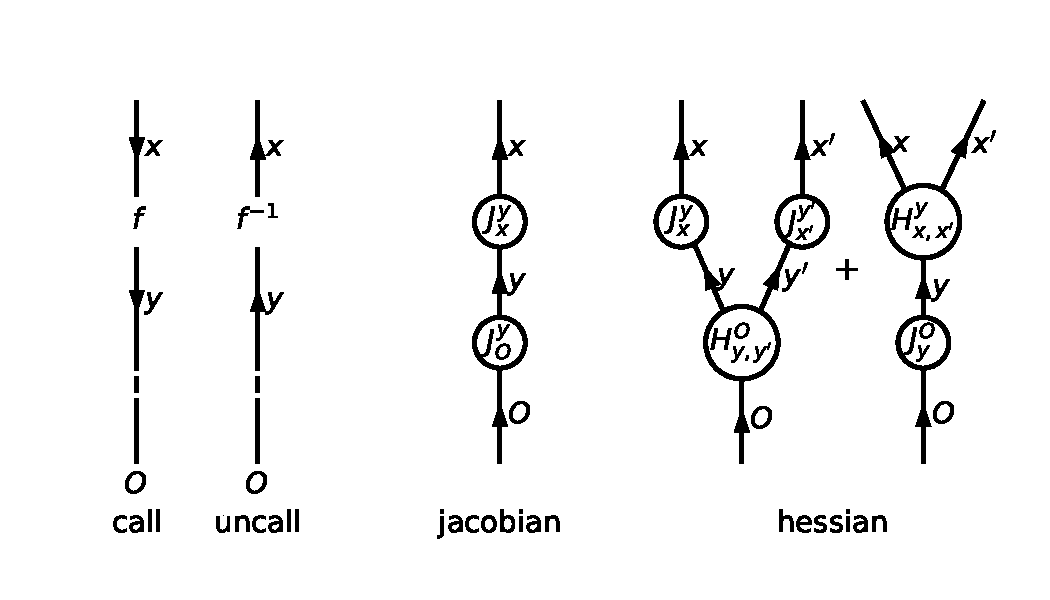
\includegraphics[width=\columnwidth,trim={0 1cm 0 1cm},clip]{images/ad.pdf}}
    \caption{Adjoint rules for Jacobians and Hessians in tensor network language.}\label{fig:ad}
\end{figure}

This approach can be easily extended to higher orders, or taylor propagation.
However, this is not the widely adopted approach to compute higher order gradients.
Althought backpropagating higher order gradients directly is exponentially faster than back propagating the computational graph for computing lower order gradients for computing higher order gradients, one has to extending the backward rules for each primitive rather than reusing existing ones.
Here, we emphasis that with instruction level AD, rewritting backward rules for primitives turns out to be not so difficult.

\subsection{Gradient on ancilla problem}
Ancilla can also carry gradients during computation, sometimes these gradients can not be uncomputed even if their parents can be uncomputed regoriously. In these case, we simply ``drop'' the gradient field instead of raising an error. In this subsection, we prove doing this is safe, i.e. does not have effect on rest parts of program.

Ancilla is the fixed point of a function, which means 
\begin{align}
    \begin{split}
    &b, y \leftarrow f(x, a)\; \text{, where } b==a\\
    &\frac{\partial b}{\partial x} = 0
    \end{split}
\end{align}

During the computation, the gradient field does not have any effect to the \texttt{value} field of variables. The key question is will the loss of gradient part in ancilla affect the reversibility of the gradient part of argument variables.
The gradient of argument variable is defined as $\frac{\partial L}{\partial x} = \frac{\partial L}{\partial y}\frac{\partial y}{\partial x} + \frac{\partial L}{\partial b}\frac{\partial b}{\partial x}$, where the second term vanish naturally.

\section{Examples}
\subsection{exp function}
The following codes implements the exp function in a reversible way

\begin{minipage}{.44\textwidth}
\begin{lstlisting}
using NiLang, NiLang.AD

@i function iexp(out!, x::T; atol::Float64=1e-14) where T
    @anc anc1 = zero(T)
    @anc anc2 = zero(T)
    @anc anc3 = zero(T)
    @anc iplus = 0
    @anc expout = zero(T)

    out! ⊕ 1.0
    @routine r1 begin
        anc1 ⊕ 1.0
        while (value(anc1) > atol, iplus != 0)
            iplus ⊕ 1
            anc2 += anc1 * x
            anc3 += anc2 / iplus
            expout ⊕ anc3
            # speudo inverse
            anc1 -= anc2 / x
            anc2 -= anc3 * iplus
            SWAP(anc1, anc3)
        end
    end

    out! ⊕ expout

    ~@routine r1
end
\end{lstlisting}
\end{minipage}

The definition of SWAP instruction can be found in \App{app:instr}.
The two lines bellow the comment \texttt{\# pseudo inverse} "uncompute" variables \texttt{anc1} and \texttt{anc2} to avalue very close to zero. Notice \texttt{*} and \texttt{/} are not exactly dual to each other.
It is reasonable to assume this inexact uncomputing will cause negligible error on final output, but harms reversibility. In the latter case, error accumulates in the whole program.
In the second for loop inside the inverse notation \texttt{\~}, we uncompute all ancilla bits rigorously.
The \texttt{while} statement takes two conditions, the precondition and postconditoin. Precondition \texttt{val(anc1) > atol} indicates when to break the forward pass and post condition \texttt{!isapprox(iplus, 0.0)} indicates when to break the backward pass.

The appendix gives another example of QR decomposition.

To obtain the gradient, one can wrap the loss with \texttt{Loss} type.

\begin{minipage}{.44\textwidth}
\begin{lstlisting}
julia> out!, x = 0.0, 1.6
(0.0, 1.6)

julia> @instr iexp'(Loss(out!), x)

julia> grad(x)
4.9530324244260555

julia> out!, x = 0.0, 1.6
(0.0, 1.6)

julia> @instr iexp''(Loss(out!), x)

julia> collect_hessian()
2×2 Array{Float64,2}:
 0.0  0.0
 0.0  4.95303
\end{lstlisting}
\end{minipage}

\texttt{iexp\textquotesingle} returns an object of type \texttt{Grad{typeof(exp)}}, it is a reversible function.
It is so short that we present the function defintion as follows

\begin{minipage}{.44\textwidth}
\begin{lstlisting}
@i function (g::Grad)(args...; kwargs...)
    @safe @assert count(x -> x isa Loss, args) == 1
    @anc iloss = 0
    @routine getiloss begin
        for i=1:length(args)
            if (tget(args,i) isa Loss, iloss==i)
                iloss += identity(i)
                (~Loss)(tget(args,i))
            end
        end
    end

    g.f(args...; kwargs...)
    GVar.(args)
    grad(tget(args,iloss)) += identity(1.0)
    (~g.f)(args...; kwargs...)

    ~@routine getiloss
end
\end{lstlisting}
\end{minipage}

The program first checks the input parameters and locate the loss variable.
Then \texttt{~Loss} unwraps the loss variable, the location of loss variable is transferred to the ancilla \texttt{iloss} of integer type.

Due to the non-locality of Hessians, we use a global tape for Hessian propagation. Whenever a new variable is created, the tape allocates a larger ring.
It is global to ease the memory allocations of ancillas, the Hessian in ancilla is important to reach correct result.
\begin{minipage}{.44\textwidth}
\begin{lstlisting}
julia> out!, x = 0.0, 1.6
(0.0, 1.6)

julia> @instr iexp''(Loss(out!), x)

julia> collect_hessian()
2×2 Array{Float64,2}:
 0.0  0.0
 0.0  4.95303
\end{lstlisting}
\end{minipage}

The final result can be obtained by calling a global function \texttt{collect\_hessian}.

\subsection{QR decomposition}

Not only simple functions, linear algebra functions 

\begin{minipage}{.44\textwidth}
\begin{lstlisting}
@i function iqr(Q, R, A::AbstractMatrix{T}) where T
    @anc anc_norm = zero(T)
    @anc anc_dot = zeros(T, size(A,2))
    @anc ri = zeros(T, size(A,1))
    for col = 1:size(A, 1)
        ri .⊕ A[:,col]
        for precol = 1:col-1
            idot(anc_dot[precol], Q[:,precol], ri)
            R[precol,col] ⊕ anc_dot[precol]
            for row = 1:size(Q,1)
                ri[row] -= anc_dot[precol] * Q[row, precol]
            end
        end
        inorm2(anc_norm, ri)

        R[col, col] += anc_norm^0.5
        for row = 1:size(Q,1)
            Q[row,col] += ri[row] / R[col, col]
        end

        ~(ri .⊕ A[:,col];
        for precol = 1:col-1
            idot(anc_dot[precol], Q[:,precol], ri)
            for row = 1:size(Q,1)
                ri[row] -= anc_dot[precol] * Q[row, precol]
            end
        end;
        inorm2(anc_norm, ri)
        )
    end
end
\end{lstlisting}
\end{minipage}

where \texttt{idot} and \texttt{inorm2} are implemented as

\begin{minipage}{.44\textwidth}
\begin{lstlisting}
@i function idot(out, v1::AbstractVector{T}, v2) where T
    @anc anc1 = zero(T)
    for i = 1:length(v1)
        anc1 ⊕ v1[i]
        CONJ(anc1)
        out += v1[i]*v2[i]
        CONJ(anc1)
        anc1 ⊖ v1[i]
    end
end

@i function inorm2(out, vec::AbstractVector{T}) where T
    @anc anc1 = zero(T)
    for i = 1:length(vec)
        anc1 ⊕ vec[i]
        CONJ(anc1)
        out += anc1*vec[i]
        CONJ(anc1)
        anc1 ⊖ vec[i]
    end
end
\end{lstlisting}
\end{minipage}

One can easily check the gradient of this naive implementation of QR decomposition is correct
\begin{minipage}{.44\textwidth}
\begin{lstlisting}
using Test
A = randn(4,4)
q = zero(A)
r = zero(A)

@i function test1(out, q, r, A)
    iqr(q, r, A)
    out ⊕ q[1,2]
end

@i function test2(out, q, r, A)
    iqr(q, r, A)
    out ⊕ r[1,2]
end

@test check_grad(test1, (Loss(0.0), q, r, A); atol=0.05, verbose=true)
@test check_grad(test2, (Loss(0.0), q, r, A); atol=0.05, verbose=true)
\end{lstlisting}
\end{minipage}

Here, the \texttt{check\_grad} function is a gradient checker function defined in \texttt{NiLangCore.ADCore}.

\subsection{Unitary Matrices}
Recurrent networks with a unitary parametrized network ease the gradient exploding and vanishing problem~\cite{Arjovsky2015,Wisdom2016,Li2016}.
Among different parametrization schemes, the most elegant one is \cite{Li2016}, which parametrized the unitary matrix with two-level unitary operations, any unitary matrix of size $N\times N$ can be parametrized by $k = N(N-1)/2$ two level unitary matrices~\cite{Li2013}. All these two-level unitary matrices can be applied in $O(1)$ time as a two register instruction.
Hence a real unitary matrix can be parametrized compactly by $k$ rotation angles, each represents a rotation operations between datas in two target parameters.


\begin{minipage}{.44\textwidth}
\begin{lstlisting}[basicstyle=\small\ttfamily,columns=fullflexible]
@i function umm!(x, θ, Nin::Int, Nout::Int)
    @anc k = 0
    for j=1:Nout
        for i=Nin-1:-1:j
            k ⊕ 1
            ROT(x[i], x[i+1], θ[k])
        end
    end

    # uncompute k
    for j=1:Nout
        for i=Nin-1:-1:j
            k ⊖ 1
        end
    end
end
\end{lstlisting}
\end{minipage}

Here, \texttt{loop j} means excuting the loop body for \texttt{j} times, it gurantes invertibility.
Loop and branching can be implemented in a more regorious way~\cite{Vieri1999} from instruction level,
however it is still an open question how to implelement loops with instruction level invertibility without compiling technic.
In the rotation instruction, \texttt{z[k]} is the rotation angle, which represents rotating data in target registers by an angle of $\theta=$ \texttt{z[k]*$\pi$}.

\begin{align}
    R(\theta)  = \begin{bmatrix}
        \cos(\theta) & - \sin(\theta)\\
        \sin(\theta)  & \cos(\theta)
    \end{bmatrix}
\end{align}

\subsubsection{The gradient}

Its backward rule is
\begin{align}
    \begin{split}
    \overline{\theta}  &= \sum\frac{\partial R(\theta)}{\partial \theta}\odot(\overline{y}x^T)\\
    &= \Tr\left[\frac{\partial R(\theta)}{\partial \theta}^T\overline{y}x^T\right]\\
    &= \Tr\left[R\left(\frac{\pi}{2}-\theta\right)\overline{y}x^T\right]
    \end{split}
\end{align}

The resulting instruction is

\begin{minipage}{.44\textwidth}
\begin{lstlisting}[basicstyle=\small\ttfamily,columns=fullflexible]
-z[k]
z[k] + pi/2
rot(gx[i], gx[ip], theta[k])
gtheta + gx[i]*x[i]
gtheta + gx[ip]*x[ip]
theta[k] - pi/2
-theta[k]

rot(gx[i], gx[ip], -pi/2)
\end{lstlisting}
\end{minipage}

In this way, the gradient is defined in a closure form.

\section{Training by consistency}
We compute the output as
\begin{equation}
    y = f(x),
\end{equation}
and we have an expected output $\hat{y}$. In traditional machine learning, we define a loss and minimize it. However, this is not how human brain works.~\cite{Hintoncomment}
Since the $\hat{y}$ is different with $y$, the network start to "think", if the output is $\hat{y}$, what should the input (including network parameters) be?
So, we feed $\hat{y}$ back to the output end of network, and inverse the tape, with the runtime information generated by the input image. The network will compute a different value to network parameters, then the network feel "confused", and chose a value between old and new values.

Let's look at the following example
\begin{minipage}{.44\textwidth}
\begin{lstlisting}[basicstyle=\small\ttfamily,columns=fullflexible]
@i function f1(out!, x, y)
    y ⊕ x
    out! -= exp(x)
    out! += exp(y)
end

@i function f2(out!, x, y)
    y ⊕ x
    out! -= exp(x)
    x -= log(-out!)
    out! += exp(y)
end

function train(f)
    loss = Float64[]
    y = 1.6
    for i=1:100
        out!, x = 0.0, 0.3
        @instr f(out!, x, y)
        push!(loss, out!)
        out! = 1.0
        @instr (~f)(out!, x, y)
    end
    loss
end
\end{lstlisting}
\end{minipage}

Loss function \texttt{f1} and \texttt{f2} computes $f(x, y) = e^{(y+x)} - e^x$ and stores the output in a new memory \texttt{out!}, the target is to find a $y$ that make the output $x$ equal to the target value $1$.
After $200$ steps training, $y$ runs into the fixed point and $x$ is equal to $1$ upto machine precision.

\begin{figure}
    \centerline{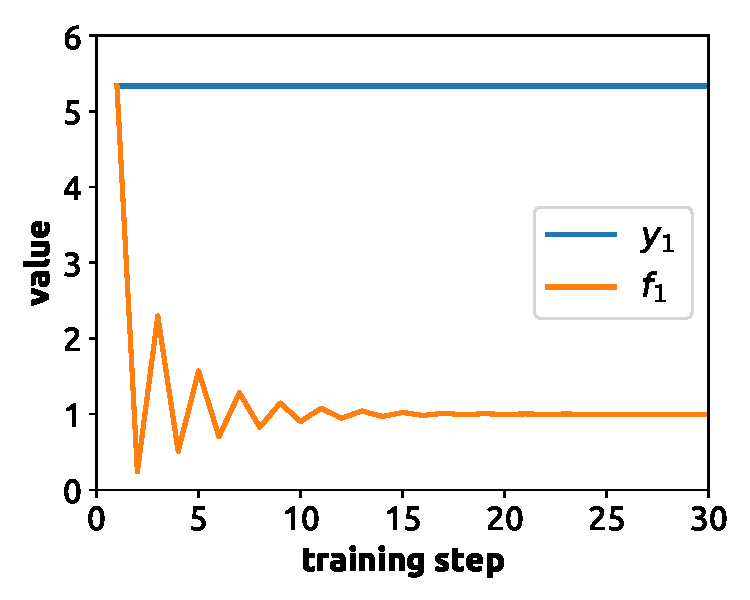
\includegraphics[width=\columnwidth,trim={0 0 0 0},clip]{images/fig1.pdf}}
    \caption{Target function value as a function of self-consistent training step.}\label{fig:invtrain}
\end{figure}

This training is similar the recursive convergence method that widely used in mathematics and physics.
However, in programming language but it has a loophole, it is vulnarable to loss of injectivity.
For example, if the result is accumulated to another variable $z += x$, and take $z$ as the loss, then the loss can not accumulated to the target value correctly since the inverse of above operation is $z -= x$ and $x$ is unchanged in the inverse run.
This is because the redundancy introduced in operation $z = z+e^x$, which keeps both $x$ and $z$, the change of $z$ shifting $z$ directly is apparently a lazier approach to fit $z$ with target value $1$, to figure out the correct causality, corresponding change in output side to $x$ and $y$ are required. This redundancy can be detected by computing the entanglement entropy (or mutual information) between two output datas. We call this type of invertibility inference, which should be avoided in this type of training. Then how shall we calculate $f(x) = e^x$ like functions, which are not partly invertible from the numeric perspective? Here we introduce the notion of "weak invertibility"
\begin{align}
    &@assert y == 0\\
    &\fl(y) += exp(\fl(x))\\
    &\fl(x) -= log(y)
\end{align}
We can keep $x$ to ensure numerical invertibility, meanwhile erase most informations inside it. Since $x$ is effectively $0$, thus no redundancy (or entanglement entropy) in output, in this way, the above training is still valid.

\subsection{Compactness of data}
Measure of compactness by entanglement entropy.
In invertible programming, we define the entanglement between output space garbage space as the compactness of information.

If the output information is compact, then we have
$(x, x_a)\rightarrow (y, y_a)$

mutual information is
\begin{align}
    I(x, y) = S(x, y) - S(x) - S(y)\\
    S(x, x_a) = S(y, y_a)\\
    I(x, x_a) = 0\\
    I(y, y_a) = S(y, y_a) - S(y_a)
\end{align}

\section{Time Space Tradeoff}
Comparing with irreversible programming, reversible programming consumes more memory.
Data have different life cycles, some are more persistent, like database, some are transiant like an ancilla variable in register that live only in several clock cycle.


\section{A Invertible Programming Style}
\section{Hardwares}
\subsection{Traditional Invertible Computing Devices}
A reversible computer, by no means refer to a computing device that every instruction or program is reversible. A better definition would be, a reversible computing device reserves the right to retract energy through uncomputing.

Like quantum computer, it should be able to reset to qubits $0$. The reset operation, sometimes can be expensive. In a quantum device, this reset operation can be done by dissipation and dicoherence (i.e. interact with environment and get thermalized). Alternatively, a immediate feedback loop can be introduced to a quantum device, where a classical computer is regarded as the dissipation source.

\subsubsection{Pendulum Design}
\textit{copy pasted begin}

It is possible to design and fabricate a fully reversible processor using resources which are comparable to a conventional microprocessor. Existing CAD tools and silicon technology are sufficient for reversible computer design.
Pendulum author demonstrated this by designing such a processor and fabricating and testing it in a commercially available CMOS process.

\textit{copy pasted end}


\subsubsection{Margolus's Billiard Ball Model Cellular Automaton (BBMCA)}
The chip is known as Flattop, not very convenient to program, but is simple, universal, reversible, and scalable.

\subsection{Quantum computers}
Fully entangled quantum systems are not easy to prepair.
For a quantum system, finding a reliable dissipation source is also not easy,
this is why the time for resetting a qubit to $0$ (or erasing a bit information) can be the bottleneck of a computing.

\section{Discussion}
One should notice the memory advantage of reversible programming to machine learning does comes from reversibility itself, but from a better data tracking strategy inspired from invertible programming.
Normally, a reversible program is not as memory efficient as its irreversible couterpart due to the additional requirement of no information loss. A naive approach that keeping track of all informations will cost an additional space $O(T)$, where $T$ stands for the excution time in a irreversible TM, the longer the program runs, the larger the memory usage is. This is exactly the approach to keeping reversibility in most machine learning packages in the market.
The point it, an reversible Turing Machine is able to trade space with time.
In some cases, it may cause polynomial overhead than its irreversible counterpart.

\subsection{Rounding errors}
\begin{align}
    a = a\cos(k\pi) - b\sin(k\pi)\\
    b = a\sin(k\pi) + b\cos(k\pi)
\end{align}
\begin{align}
    \begin{split}
    \epsilon_a &= -a\sin(\theta)\theta\epsilon - b\cos(\theta)\theta\epsilon + a\epsilon\cos(\theta) - b\epsilon\sin(\theta)\\
            &\sim \max(a ,b)\epsilon
    \end{split}
\end{align}
The error accumulates linearly as the number of floating point operations, for a $N\times N$ unitary matrix, each number is operated $~N$ times.
In a double precision computation, the rounding errors in unitary matrix multiplication will probably not have a substaintial effect on resersibility.

\subsection{Performance}
Todays CPU are starving, that is, the memory access is more time consuming than actual computational time.
How the extra uncomputing operations affect the performance can not be easily estimated by counting the number of instructions.

In the simplest g-segment trade off scheme~\cite{}, it takes $Time(T) = T^{\log _g(4g-2)}$ and $Space(T) = (g-1)S\log_g T$.
In practise, there are more practical trading off schemes that works much better in practise.~\cite{}
Checkpointing ~\cite{Chen2016}.
In our work, especially in the \texttt{iexp} example, we show the the irreversibility of $*$ and $/$ can be mitigated.

\subsection{Reversibility and renormalization level}
%\begin{definition}
    For an algorihms, the renormalization level of a program is the logarithm of the ratio between length of reversible instructions and irreversible instruction.
%\end{definition}

\subsection{Quantum Computing}
One of the fundamental difficulty of building a quantum computer is, unlike a classical state, an unknown quantum state can not be copied.
A quantum state in a environment will decoherence and can not be recovered, this underlines the simulation nature of a quantum device.
In the era of noisy intermediate sized quantum devices, more and more people are switching to classical-quantum hybrid devices, where a quantum device plays the role of a programmable simulator.
Reversible computing does not enjoy the supremacy from quantum entanglement, nor the quantum limitations of non-cloning.
Only the limitation of reversibility is retained, reversibility comes from the fact that micro scopic processes are all unitary.
Irreversibility can only come from the interaction with classical devices, like environment induces decaying, qubit state resetting, measurements and classical feedbacks to quantum devices. These are rare resources in microscopic world as well as one of the most difficult part to implement in a practical device.

Quantum gates can possiblely simplify reversible instructions design, e.g. the quantum fourier transformation based adder.
A classical in, classical out algorithm can find a quantum shortcut.
With respect to this fact, it is reasonable to believe there would be a classical-quantum intermediate statge of computing,
the reversible computing that bridge the gap between classical bits and fully entangled qubits.
Although weaker than both, but with a killer application of instruction level automatic differentiation.
By introducing quantum entanglement little by little, we will have faster instructions, faster algorithms and finally have an application that has genuine quantum advantage.

\section{acknowledgments}
The authors are supported by the National Natural Science Foundation of China under the Grant No.~11774398, the Strategic Priority Research Program of Chinese Academy of Sciences Grant No.~XDB28000000 and the research funding from Huawei Technologies under the Grant No.~YBN2018095185.

\bibliographystyle{apsrev4-1}
\bibliography{invc}

\pagebreak
\appendix

\section{NiLang Grammar}\label{app:grammar}

Terminologies
\begin{itemize}
    \item $ident$, symbols
    \item $num$, numbers
    \item $\epsilon$, empty statement
    \item $JuliaExpr$, native julia expression,
    \item $[$ $]$,  zero or one repetitions.
\end{itemize}

\begin{minipage}{0.3\textwidth}
    \small
\begin{bnf*}
    \bnfprod{Stmts}{\bnfsp \bnfes}\\
    \bnfmore{\bnfor \bnfpn{Stmt}}\\
    \bnfmore{\bnfor \bnfpn{Stmts} \bnfsp \bnfpn{Stmt}}\\
    \bnfprod{Stmt}{\bnfpn{BlockStmt}}\\
    \bnfmore{\bnfor \bnfpn{IfStmt}}\\
    \bnfmore{\bnfor \bnfpn{WhileStmt}}\\
    \bnfmore{\bnfor \bnfpn{ForStmt}}\\
    \bnfmore{\bnfor \bnfpn{InstrStmt}}\\
    \bnfmore{\bnfor \bnfpn{RevStmt}}\\
    \bnfmore{\bnfor \bnfpn{@anc} \bnfsp \bnfpn{Stmt}}\\
    \bnfmore{\bnfor \bnfpn{@routine} \bnfsp \bnfpn{Stmt}}\\
    \bnfmore{\bnfor \bnfpn{@safe} \bnfsp \bnftd{$JuliaExpr$}}\\
    \bnfmore{\bnfor \bnfpn{CallStmt}}\\
    \bnfprod{BlockStmt}{\bnftd{begin} \bnfsp \bnfpn{Stmts} \bnfsp \bnftd{end}}\\
    \bnfprod{RevCond}{\bnftd{(} \bnfsp \bnftd{$JuliaExpr$} \bnfsp \bnftd{,} \bnfsp \bnftd{$JuliaExpr$} \bnfsp \bnftd{)}}\\
    \bnfprod{IfStmt}{\bnftd{if} \bnfsp \bnfpn{RevCond} \bnfsp \bnfpn{Stmts} \bnfsp \bnfts{[} \bnftd{else} \bnfsp \bnfpn{Stmts}\bnfts{]} \bnfsp \bnftd{end}}\\
    \bnfprod{WhileStmt}{\bnftd{while} \bnfsp \bnfpn{RevCond} \bnfsp \bnfpn{Stmts} \bnfsp \bnftd{end}}\\
    \bnfprod{Range}{\bnftd{$JuliaExpr$} \bnfsp \bnftd{:} \bnfsp \bnftd{$JuliaExpr$} \bnfsp \bnfts{[} \bnftd{:} \bnfsp \bnftd{$JuliaExpr$}\bnfts{]}}\\
    \bnfprod{ForStmt}{\bnftd{for} \bnfsp \bnftd{ident} \bnfsp \bnftd{=} \bnfsp \bnfpn{Range} \bnfsp \bnfpn{Stmts} \bnfsp \bnftd{end}}\\
    \bnfprod{CallStmt}{\bnftd{$JuliaExpr$} \bnfsp \bnftd{(} \bnfsp \bnfts{[} \bnfpn{DataViews}\bnfts{]} \bnfsp \bnftd{)}}\\
    \bnfprod{Constant}{\bnftd{num} \bnfor \bnftd{$\pi$}}\\
    \bnfprod{InstrBinOp}{\bnftd{+=} \bnfor \bnftd{-=} \bnfor \bnftd{$\veebar$=}}\\
    \bnfprod{InstrTrailer}{\bnfts{[} \bnftd{.}\bnfts{]} \bnfsp \bnftd{(} \bnfsp \bnfts{[} \bnfpn{DataViews}\bnfts{]} \bnfsp \bnftd{)}}\\
    \bnfprod{InstrStmt}{\bnfpn{DataView} \bnfsp \bnfpn{InstrBinOp} \bnfsp \bnftd{ident} \bnfsp \bnfts{[} \bnfpn{InstrTrailer}\bnfts{]}}\\
    \bnfprod{RevStmt}{\bnftd{$\sim$} \bnfsp \bnfpn{Stmt}}\\
    \bnfprod{@routine}{\bnftd{@routine} \bnfsp \bnftd{ident} \bnfsp \bnfpn{Stmt}}\\
    \bnfprod{AncArg}{\bnftd{ident} \bnfsp \bnftd{=} \bnfsp \bnftd{$JuliaExpr$}}\\
    \bnfprod{@anc}{\bnftd{@anc} \bnfsp \bnfpn{AncArg}}\\
    \bnfmore{\bnfor \bnftd{@deanc} \bnfsp \bnfpn{AncArg}}\\
    \bnfprod{@safe}{\bnftd{@safe} \bnfsp \bnftd{$JuliaExpr$}}\\
    \bnfprod{DataViews}{\bnfsp \bnfes}\\
    \bnfmore{\bnfor \bnfpn{DataView}}\\
    \bnfmore{\bnfor \bnfpn{DataViews} \bnfsp \bnftd{,} \bnfsp \bnfpn{DataView}}\\
    \bnfprod{DataView}{\bnfpn{DataView} \bnfsp \bnftd{[} \bnfsp \bnftd{$JuliaExpr$} \bnfsp \bnftd{]}}\\
    \bnfmore{\bnfor \bnfpn{DataView} \bnfsp \bnftd{.} \bnfsp \bnftd{ident}}\\
    \bnfmore{\bnfor \bnftd{$JuliaExpr$} \bnfsp \bnftd{(} \bnfsp \bnfpn{DataView} \bnfsp \bnftd{)}}\\
    \bnfmore{\bnfor \bnfpn{Constant}}\\
    \bnfmore{\bnfor \bnftd{ident}}\\
\end{bnf*}

\end{minipage}

Dataview is a special surjective mapping of parent data, e.g. a field of an object.
The dataview can feedback to parent data with the 
\texttt{chfield} method, so that the modified object can generate desired dataview.

\section{Instruction Table}\label{app:instr}
Even though \texttt{$\oplus$}, \texttt{$\oplus(*)$}, \texttt{$\oplus(/)$} and their reverse together with control flows are sufficient to write an arbituary differentiable program.
For convinience we provide more,
\begin{table}[h!]\centering
\begin{minipage}{\columnwidth}
\ra{1.3}
    \scalebox{1.0}{
        \begin{tabularx}{\textwidth}{X X}\toprule
            ${\rm SWAP}(a, b) \rightarrow b, a$\\
            ${\rm ROT}(a, b, \theta) \rightarrow a \cos\theta - b\sin\theta, b \cos\theta + a\sin\theta, \theta$\\
            ${\rm IROT}(a, b, \theta) \rightarrow a \cos\theta + b\sin\theta, b \cos\theta - a\sin\theta, \theta$\\
            $y \pluseq a^\wedge b \rightarrow y+a^b, a, b$\\
            $y \pluseq \exp(x) \rightarrow y+e^x, x$\\
            $y \pluseq \log(x) \rightarrow y+\log x, x$\\
            $y \pluseq \sin(x) \rightarrow y+\sin x, x$\\
            $y \pluseq \cos(x) \rightarrow y+\cos x, x$\\
            $y \pluseq {\rm abs}(x) \rightarrow y+ |x|, x$\\
            ${\rm NEG}(y) \rightarrow -y$\\
            ${\rm CONJ}(y) \rightarrow y'$\\
            \bottomrule
        \end{tabularx}
    }
    \caption{A collection of reversible instructions.}\label{tbl:revstatements}
\end{minipage}
\end{table}

\section{Computing Fibonacci Sequence}\label{app:fib}
\begin{minipage}{.44\textwidth}
\begin{lstlisting}
function fib(n)
    if n > 2
        fib(n-1) + fib(n-2)
    else
        one(n)
    end
end
\end{lstlisting}
\end{minipage}

\begin{minipage}{.44\textwidth}
\begin{lstlisting}
@i function rfib(out, n::T) where T
    @anc n1 = zero(T)
    @anc n2 = zero(T)
    n1 ⊕ n
    n1 ⊖ 1.0
    n2 ⊕ n
    n2 ⊖ 2.0
    if (value(n) <= 2, ~)
        out ⊕ 1.0
    else
        rfib(out, n1)
        rfib(out, n2)
    end
    n1 ⊖ n
    n1 ⊕ 1.0
    n2 ⊖ n
    n2 ⊕ 2.0
end
\end{lstlisting}
\end{minipage}


\section{Julia based DSL implementation details}

Macro `invfunc` defines a invertible function, ancillas are binded to a function, since ancillas are umcomputed to $0$ at the end of call, so that it can be used repeatedly in a function, it is like a class variable in a class, with no side effects.

Some variables can be uncomputed to $0$, but we choose not to for performance reason. For example
\texttt{infer!(argmax, i, x)} which computes the location of maximum value in $x$ and store the output to $i$, if we uncompute it, it doubles additional computational time. Here, we trade off the memory with computation time. As a result, we must feed \texttt{imax} to the function, so that this variable can be manipulated in outer scopes.

%\end{multicols}
\end{document}
